\documentclass[10pt, landscape]{article}
\usepackage[scaled=0.92]{helvet}
\usepackage{calc}
\usepackage{multicol}
\usepackage{ifthen}
\usepackage[a4paper,margin=5mm,landscape]{geometry}
\usepackage{amsmath,amsthm,amsfonts,amssymb}
\usepackage{color,graphicx,overpic}
\usepackage{hyperref}
\usepackage{newtxtext} 
\usepackage{enumitem}
\usepackage{amssymb}
\usepackage[table]{xcolor}
\usepackage{vwcol}
\usepackage{tikz}
\usetikzlibrary{arrows.meta}
\usetikzlibrary{calc}
\usepackage{mathtools}
\usepackage{nicematrix}
\usepackage[T1]{fontenc} %%% <--- NOTE THIS
% for relations
\usepackage{cancel}
\usepackage{ mathrsfs }
\usepackage{listings}
\usepackage{background}
\setlist{nosep}

\usepackage{etoolbox}
\makeatletter
\preto{\@verbatim}{\topsep=0pt \partopsep=0pt }
\makeatother

\backgroundsetup{
scale=1,
color=black,
opacity=0.4,
angle=0,
contents={%
  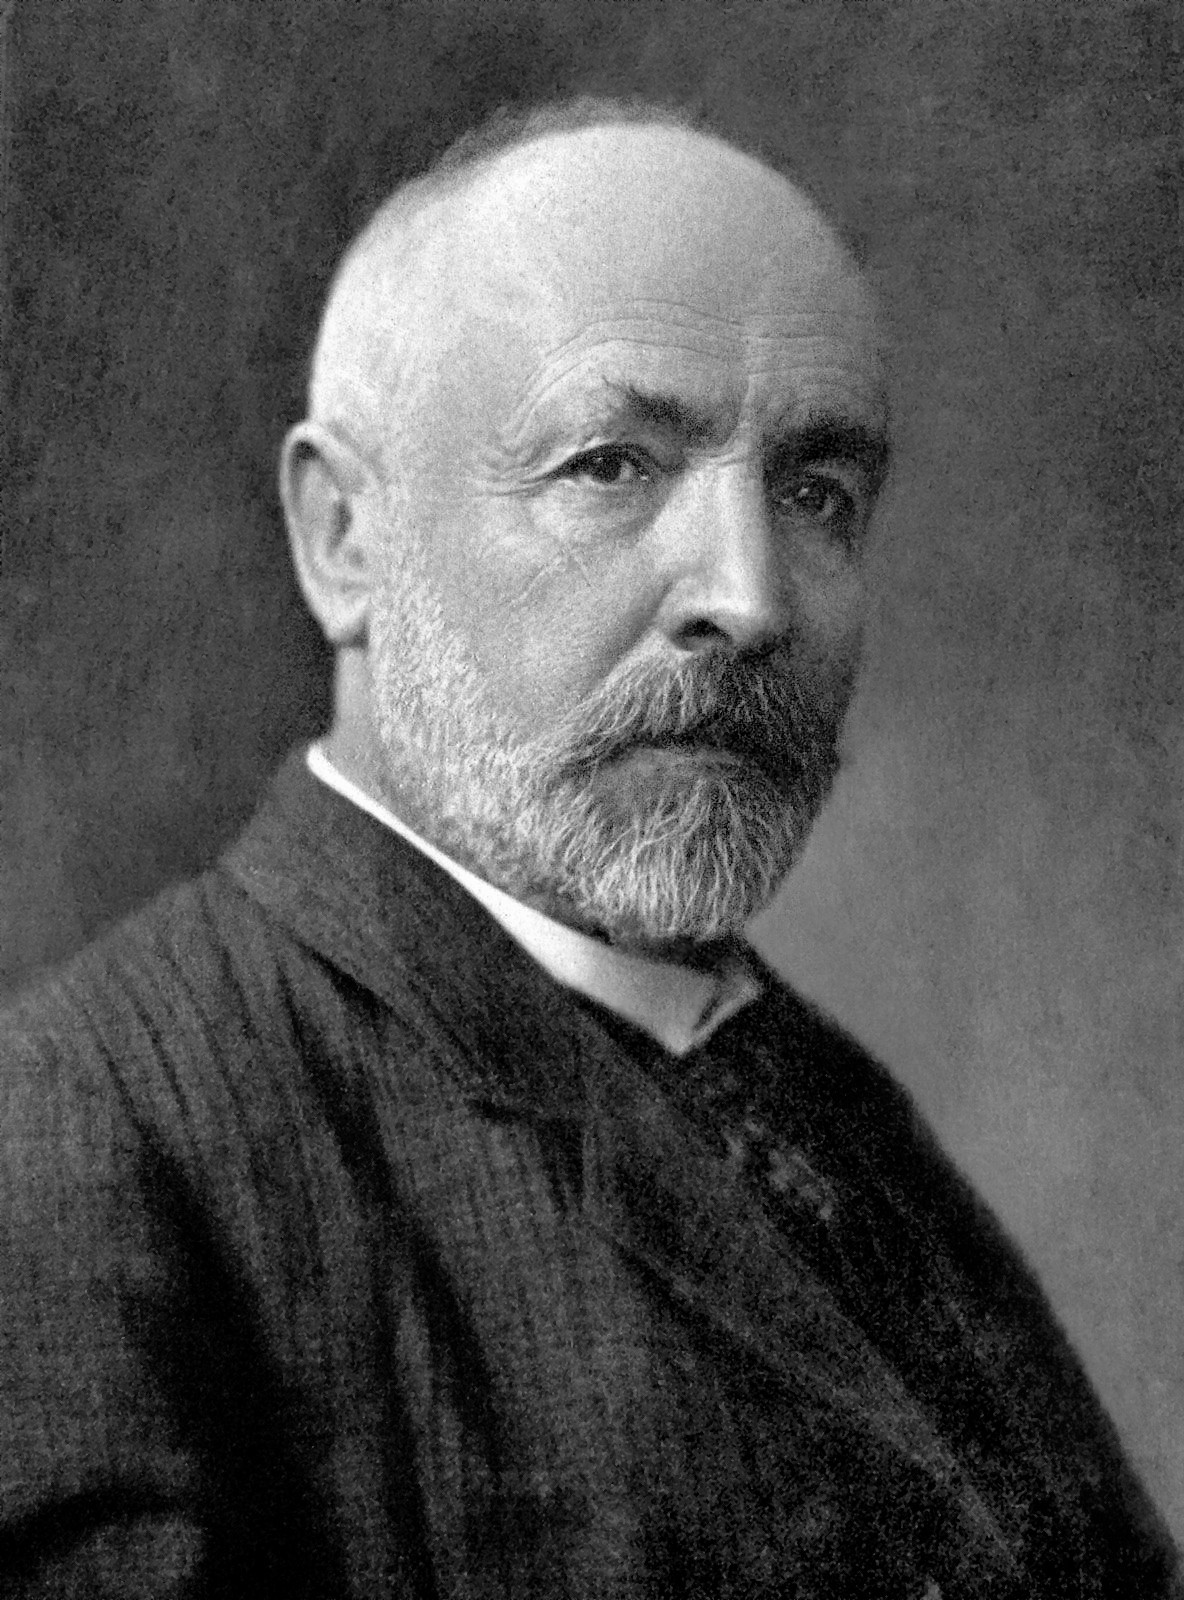
\includegraphics[width=0.5\paperwidth,height=\paperheight]{cantor.jpg}
  
\includegraphics[width=0.5\paperwidth,height=\paperheight]{dilip.jpg}
  }%
}

\pdfinfo{
  /Title (MA3205.pdf)
  /Creator (TeX)
  /Producer (pdfTeX 1.40.0)
  /Author (Seamus)
  /Subject (Example)
  /Keywords (pdflatex, latex,pdftex,tex)}

\lstset{language=Java,keywordstyle={\bfseries \color{black}}}

% Turn off header and footer
\pagestyle{empty}

\newenvironment{tightcenter}{%
  \setlength\topsep{0pt}
  \setlength\parskip{0pt}
  \begin{center}
}{%
  \end{center}
}

% redefine section commands to use less space
\makeatletter
\renewcommand{\section}{\@startsection{section}{1}{0mm}%
                                {-1ex plus -.5ex minus -.2ex}%
                                {0.5ex plus .2ex}%x
                                {\normalfont\large\bfseries}}
\renewcommand{\section}{\@startsection{section}{2}{0mm}%
                                {-1explus -.5ex minus -.2ex}%
                                {0.5ex plus .2ex}%
                                {\normalfont\normalsize\bfseries}}
\renewcommand{\subsection}{\@startsection{subsection}{3}{0mm}%
                                {-1ex plus -.5ex minus -.2ex}%
                                {1ex plus .2ex}%
                                {\normalfont\small\bfseries}}%
\renewcommand{\familydefault}{\sfdefault}
\renewcommand\rmdefault{\sfdefault}
% makes nested numbering (e.g. 1.1.1, 1.1.2, etc)
\renewcommand{\labelenumii}{\theenumii}
\renewcommand{\theenumii}{\theenumi.\arabic{enumii}.}
\renewcommand\labelitemii{•}
%  for logical not operator
\renewcommand{\lnot}{\mathord{\sim}}
\renewcommand{\bf}[1]{\textbf{#1}}
\newcommand{\abs}[1]{\vert #1 \vert}
\newcommand{\Mod}[1]{\ \mathrm{mod}\ #1}

\makeatother
\definecolor{myblue}{cmyk}{1,.72,0,.38}
\everymath\expandafter{\the\everymath \color{myblue}}
% Define BibTeX command
\def\BibTeX{{\rm B\kern-.05em{\sc i\kern-.025em b}\kern-.08em
    T\kern-.1667em\lower.7ex\hbox{E}\kern-.125emX}}
\let\iff\leftrightarrow
\let\Iff\Leftrightarrow
\let\then\rightarrow
\let\Then\Rightarrow

% Don't print section numbers
\setcounter{secnumdepth}{0}

\setlength{\parindent}{0pt}
\setlength{\parskip}{0pt plus 0.5ex}
%% this changes all items (enumerate and itemize)
\setlength{\leftmargini}{0.5cm}
\setlength{\leftmarginii}{0.5cm}
\setlist[itemize,1]{leftmargin=2mm,labelindent=1mm,labelsep=1mm}
\setlist[itemize,2]{leftmargin=4mm,labelindent=1mm,labelsep=1mm}

%My Environments
\newtheorem{example}[section]{Example}
% -----------------------------------------------------------------------

\begin{document}
\raggedright
\footnotesize
\begin{multicols*}{3}

% multicol parameters
% These lengths are set only within the two main columns
\setlength{\columnseprule}{0.25pt}
\setlength{\premulticols}{1pt}
\setlength{\postmulticols}{1pt}
\setlength{\multicolsep}{1pt}
\setlength{\columnsep}{2pt}

\begin{center}
    \fbox{%
        \parbox{0.8\linewidth}{\centering \textcolor{black}{
            {\Large\textbf{MA3205}}
            \\ \normalsize{AY24/25 Sem 2}}
            \\ {\footnotesize \textcolor{myblue}{by ngmh}} 
        }%
    }
\end{center}

\section{1. Sets and Operations}
\textbf{A1.1 Axiom of Extensionality} $\forall x\ [x \in A \Longleftrightarrow x \in B]$

\textbf{D1.6 Subcollection} $A \subseteq B$ if $\forall x\ [x \in A \Rightarrow x \in B]$

\textbf{D1.7 Empty Set} $x$ is empty if $\forall y\ [y \notin x]$

\textbf{F1.8} If $x = \emptyset$ and $A$ is a collection then $x \subseteq A$

\textbf{F1.9} If $x=\emptyset$ and $y=\emptyset$, $x=y$

\textbf{D1.11 Basic Operations}
\begin{enumerate}
    \item $x \cup y = \{z : z\in x \lor z \in y\}$
    \item $x \cap y = \{z : z\in x \land z \in y\}$
    \item $x\ \backslash\ y = \{z : z\in x \land z \notin y\}$
    \item $x\ \triangle\ y = (x\ \backslash \ y)\ \cup (y\ \backslash \ x)$
    \item $\mathcal{P}(x)=\{z:z\subseteq x\}$
\end{enumerate}

\textbf{L1.12 Properties}
\begin{enumerate}
    \item $x \cup y = y \cup x$
    \item $x \cap y = y \cap x$
    \item $x \cup (y \cup z) = (x \cup y) \cup z$
    \item $x \cap (y \cap z) = (x \cap y) \cap z$
    \item $x \cup (y \cap z) = (x \cup y) \cap (x \cup z)$
    \item $x \cap (y \cup z) = (x \cap y) \cup (x \cap z)$
    \item $x\ \backslash\ (y \cup z) = (x\ \backslash\ y) \cap (x\ \backslash\ z)$
    \item $x\ \backslash\ (y \cap z) = (x\ \backslash\ y) \cup (x\ \backslash\ z)$
\end{enumerate}

\textbf{D1.13 Union and Intersection}

$\bigcup A = \{x: \exists y \ [y \in A \land x \in y]\}$

$\bigcap A =
    \left\{
    \begin{array}{lr}
      \emptyset & \text{if $A=\emptyset$} \\
      \{x:\forall y \ [y \in A \Rightarrow x \in y]\} & \text{otherwise} \\
    \end{array}
    \right.
$

\textbf{E1.16 Symmetric Difference}
\begin{enumerate}
    \item $(X\ \triangle\ Y)\ \triangle \ Z = X \ \triangle\ (Y \ \triangle \ 
Z)$
    \item $X \ \triangle \ X = \emptyset$
    \item $X \ \triangle \ Y = Y \ \triangle \ X$
    \item $X \ \triangle \ \emptyset = X$
\end{enumerate}

\textbf{E1.18} $X \cap (Y \ \triangle \ Z) = (X \cap Y) \ \triangle \ (X \cap Z)$


\section{2. Pairing, Products, and Relations}
\textbf{D2.1 Ordered Pair} $\langle a, b \rangle = \{\{a\},\{a,b\}\}$

\textbf{L2.2} $\langle x, y \rangle = \langle a, b \rangle$ iff $x=a \land y = b$

\textbf{D2.3 Cartesian Product} $A \times B=\{z:\exists a \in A\  \exists b \in B \ [z = \langle a, b \rangle]\}$, $A^2 = A \times A$

\textbf{E2.5} Define $pair(a,b)=\{a, \{a, b\}\}$. Assuming we cannot have $A\in B\in A$, $pair(a,b)=pair(x,y)$ iff $a=x \land b = y$

\textbf{D2.6 Relation} A relation is a collection of ordered pairs.
\begin{enumerate}
    \item $R$ is a relation if $\forall x \in R \ \exists a\ \exists b\ [x=\langle a, b \rangle]$
    \item $R$ is a relation on $A$ if $R \subseteq A \times A$
    \item $dom(R)=\{a:\exists b \ [\langle a, b \rangle \in R]\}$
    \item $ran(R)=\{b:\exists a \ [\langle a, b \rangle \in R]\}$
    \item $R^{-1}=\{x:\exists a \ \exists b \ [\langle a, b \rangle \in R \land x = \langle b, a \rangle]\}$
\end{enumerate} 

\textbf{D2.8 Function} A function is a relation where no  two elements have the same first coordinate.
\begin{enumerate}
    \item 
    $\forall a,b,c \ [(\langle a, b \rangle \in f \land \langle a, c \rangle \in f) \Rightarrow b=c]$
    \item $f:A \rightarrow B$ if $f$ is a function, $dom(f)=A$ and $ran(f) \subseteq B$
\end{enumerate}

\textbf{F2.9} If $R$ is a relation and $S \subseteq R$, then $S$ is a relation. If $f$ is a function and $g \subseteq f$, then $g$ is a function.

\textbf{D2.10} $R$ restricted to $A$: $R \restriction A=R \cap (A \times ran(R))$

\textbf{F2.11} $f \restriction A$ is a function. If $A \subseteq dom(f)$, then $dom(f \restriction A) = A$

\textbf{D2.12} Image of $A$ under $R$: $Im_R(A)=\{b:\exists a \in A \ [\langle a, b \rangle \in R]\}$. If $f$ is a function, for any $a \in dom(f)$ $f(a)$ denotes the unique $b$ such that $\langle a, b \rangle \in f$

\textbf{D2.14} $Im_{f^{-1}}(B)=\{a:\exists b \in B \ [\langle b, a \rangle \in f^{-1}]\}=\{a:\exists b \in B \ [\langle a, b \rangle \in f]\}=\{a:a \in dom(f) \land f(a) \in B\}$

\textbf{L2.15} $Im_R(\bigcup A)=\bigcup\{I:\exists a \in A \ [I=Im_R(a)]\}$

\textbf{L2.16} If for any $x$ and $z$, if $x \neq z$ then $Im_R(\{x\})\cap Im_R(\{z\})=\emptyset$, then
\begin{enumerate}
    \item $Im_R(\bigcap A)=\bigcap\{I:\exists a \in A \ [I=Im_R(a)]\}$
    \item $Im_R(B \ \backslash \ A)=Im_R(B)\ \backslash \ Im_R(A)$
\end{enumerate}

\textbf{C2.17} For any function and sets,
\begin{enumerate}
    \item $Im_{f^{-1}}(\bigcup A)=\bigcup\{I:\exists a \in A \ [I=Im_{f^{-1}}(a)]\}$
    \item $Im_{f^{-1}}(\bigcap A)=\bigcap\{I:\exists a \in A \ [I=Im_{f^{-1}}(a)]\}$
    \item $Im_{f^{-1}}(B \ \backslash \ A)=Im_{f^{-1}}(B) \ \backslash \ Im_{f^{-1}}(A)$
\end{enumerate}

\textbf{D2.18} $f$ as composed with $g$: $g \circ f=\{x:\exists a \ \exists b \ \exists c \ [\langle a,b \rangle \in f \land \langle b, c \rangle \in g \land x = \langle a, c \rangle]\}$

\textbf{L2.19} If $f,g,h$ are functions then
\begin{enumerate}
    \item $g \circ f$ is a function
    \item If $f:A\rightarrow B$ and $g:B\rightarrow C$, then $g \circ f: A \rightarrow C$
    \item $h \circ (g \circ f)=(h \circ g) \circ f$
\end{enumerate}

\textbf{D2.20 Injection 
 / Surjection / Bijection} Consider $f:A \rightarrow B$
\begin{enumerate}
    \item $1-1$ / Injection: $\forall a, a' \in A \ [f(a)=f(a') \Rightarrow a = a']$
    \item Onto / surjection: $ran(f)=B$
    \item Bijection: $1-1$ and Onto
\end{enumerate}

\textbf{D2.21} $X^Y=\{f:f \ \text{is a function} \land f: Y \rightarrow X\}$

\textbf{L2.22} If $f:A \rightarrow B$ is $1-1$ and onto, then $f^{-1}:B \rightarrow A$ is $1-1$ and onto.

\textbf{E2.23} It is possible that $Im_f(a \cap b) \neq Im_f(a) \cap Im_f(b)$

\textbf{E2.24} If $f$ is $1-1$, $Im_f(\bigcap A) = \bigcap\{Im_f(a):a \in A\}$ and $Im_f(B \ \backslash \ A)=Im_f(B)\ \backslash \ Im_f(A)$

\textbf{2.27} The following are equivalent
\begin{enumerate}
    \item $\forall x, z \ [x \neq z \Rightarrow Im_R(\{x\}) \cap Im_R(\{z\}) = \emptyset]$
    \item $R^{-1}$ is a function
\end{enumerate}

\textbf{CV2.28 Functions as sequences} Suppose $dom(f)=I$. $f=\langle A_i:i \in I \rangle=\{x:\exists i \in I \ [x=\langle i, A_i \rangle]\}$. $\forall i \in I, f(i) =A_i$.

\textbf{CV2.29}
\begin{enumerate}
    \item $Im_f(A)=\{f(a):a \in A \cap dom(f)\}$. If $A\subseteq dom(f)$, then $Im_f(A)=\{f(a): a \in A\}$
    \item If $dom(f)=A \times B$, $f(\langle a, b \rangle)=f(a,b)$
\end{enumerate}

\textbf{CV2.30} Suppose $F$ is a function, $x \in dom(F)$, and $F(x)$ is also a function. Then if $y \in dom(F(x))$, $F(x)(y)=(F(x))(y)$.

\textbf{CV2.32} If $F=\langle A_i:i \in I\rangle$, then $\bigcup ran(F)=\bigcup_{i\in I}A_i$, similarly for $\bigcap ran(F)$

\textbf{CV2.33} To specify a function $f$ with domain $I$, it is enough to specify $f(i)$ for each $i \in I$. $f=\{z:\exists i \in I \ \exists x \ [z=\langle i, x \rangle \land x\ \text{satisfies property $P$ w.r.t}\ i]\}$. If there is a unique object satisfying $P$ for each $i$, then $f$ is a function and $dom(f)=I$.

\textbf{EP2.34} Define $F: \mathbb{N}^\mathbb{N} \rightarrow \mathbb{N}^\mathbb{N}$. For $f \in \mathbb{N}^\mathbb{N}$, we must specify $F(f) \in \mathbb{N}^\mathbb{N}$. We must specify $F(f)(n)\in \mathbb{N}$ for each $n \in \mathbb{N}$. For example, $F(f)(n)=f(n)+1$. Then $F(f)=\{\langle n, f(n)+1 \rangle : n \in \mathbb{N}\}$ and $F=\{\langle f, \{\langle n, f(n)+1 \rangle : n \in \mathbb{N}\}\rangle  : f \in \mathbb{N}^\mathbb{N}\}$. Similarly, define $\mathcal{F} : (\mathbb{N}^\mathbb{N})^\mathbb{N} \rightarrow \mathbb{N}^\mathbb{N}$. For $F\in (\mathbb{N}^\mathbb{N})^\mathbb{N}$, we must specify $\mathcal{F}(F)\in \mathbb{N}^\mathbb{N}$ by specifying $\mathcal{F}(F)(n)$ for each $n$. Since $F$ is a function with domain $\mathbb{N}$, $F(i)$ is defined for all $i \leq n$ and $F(i)\in \mathbb{N}^\mathbb{N}$. So $F(i)(n) \in \mathbb{N}$. Set $\mathcal{F}(F)(n)=max\{F(i)(n) : i \leq n\}$. $\mathcal{F}(F)$ eventually dominates $\{F(n):n \in \mathbb{N}\}$.

\textbf{EP2.35} Let $I$ be a set, $\langle J_i : i \in I \rangle$ be a sequence of sets, and $\langle A_{i, j} : j \in J_i$ be a sequence of sets. Define $X=\{\bigcup_{j\in J_i}A_{i, j}: i \in I\}$. First define $F$ with $dom(F)=I$. For each $i \in I$, $F(i) = \bigcup_{j \in J_i}A_{i, j}$. $X=Im_F(I)=ran(F)$. $\bigcap X=\bigcap_{i \in I}\bigcup_{j \in J_i}A_{i, j}$.

\textbf{EP2.36} There is a biection $F:\mathcal{P}(X)\rightarrow \{0,1\}^X$. We must specify $F(a)$ for each $a \in \mathcal{P}(X)$; a function with $dom(F(a))=X$ and $ran(F(a)) \subseteq\{0, 1\}$. It is enough to specify $F(a)(x)$ for each $x \in X$.

$F(a)(x) =
    \left\{
    \begin{array}{lr}
      0 & \text{if $x \in A$} \\
      1 & \text{if $x \notin A$} \\
    \end{array}
    \right.
$ which is $1-1$ and onto.

\textbf{D2.37 Cartesian Product} Let $F$ be a function with $dom(F)$ as a set. $\prod F=\{f:f \ \text{is a function} \land dom(f) = dom(F) \land \forall x \in dom(F) \ [f(x) \in F(x)]\}$. If $F=\langle A_i : i \in I \rangle$, then $\prod F = \prod_{i \in I}A_i = \{f: f \ \text{is a function} \land dom(f)=I \land \forall i \in I\ [f(i) \in A_i]\}$

\textbf{A2.38 Axiom of Choice} If $\langle A_i : i \in I \rangle$ is a sequence of sets such that $\forall i \in I \ [A_i \neq \emptyset]$, then $\prod_{i \in I} A_i \neq \emptyset$

\textbf{D2.40 Directed Collection} $G$ is directed if $\forall a, b \in G \ \exists c \in G \ [a\subseteq c \land b \subseteq c]$

\textbf{L2.41} If $G$ is a directed collection of functions, $f=\bigcup G$ is a function. $dom(f)=\bigcup\{dom(\sigma):\sigma \in G\}$ and $ran(f)=\bigcup\{ran(\sigma) : \sigma \in G\}$

\textbf{T2.47 Generalised De Morgan's} (Requires \textbf{Axiom of Choice}) Let $I$ be a set, and $\langle J_i: i \in I \rangle$ be a sequence of sets. Suppose $I \neq \emptyset$ and $\forall i \in I \ [J_i \neq \emptyset]$. For each $i \in I$, let $\langle A_{i, j} : j \in J_i \rangle$ be a sequence of sets.
\begin{enumerate}
    \item $\bigcup_{i \in I} \bigcap_{j \in J_i}A_{i,j}=\bigcap\{\bigcup_{i\in I}A_{i,f(i)}:f\in \prod_{i \in I}J_i\}$
    \item $\bigcap_{i \in I} \bigcup_{j \in J_i}A_{i,j}=\bigcup\{\bigcap_{i\in I}A_{i,f(i)}:f\in \prod_{i \in I}J_i\}$
    \item $\prod_{i \in I}(\bigcup_{j\in J_i}A_{i,j})=\bigcup\{\prod_{i \in I}A_{i, f(i)}:f\in\prod_{i\in I} J_i\}$
    \item $\prod_{i \in I}(\bigcap_{j\in J_i}A_{i,j})=\bigcap\{\prod_{i \in I}A_{i, f(i)}:f\in\prod_{i\in I} J_i\}$
\end{enumerate}

\textbf{T2.48} Fix $n \geq 1$, Let $X$ be a set and $A_1, ..., A_n$ be subsets of $X$. There are at most $2^{2^n}$ sets that can be formed using $X \ \backslash \ ., \cup,$ and $\cap$.
\begin{enumerate}
    \item Redefine $\bigcap \emptyset = X$
    \item Let $S=\{0, 1\}^{\{1, ..., n\}}$, then $|S|=2^n$
    \item For each $\sigma \in S$ define $b_\sigma=(\bigcap\{A_i:\sigma(i)=0\})\cap(\bigcap\{X\ \backslash \ A_i:\sigma(i)=1\})$
    \item For each $a\in \mathcal{P}(S)$ let $c_a=\bigcup\{b_\sigma:\sigma\in a\}$
    \item Let $\mathcal{B}=\{c_a:a\in \mathcal{P}(S)\}$. $|\mathcal{B}|\leq|\mathcal{P}(S)|=2^{2^n}$
    \item \textbf{CL2.49} For each $1 \leq i \leq n$, $A_i\in \mathcal{B}$
    \item \textbf{CL2.50} For any $a, b \in \mathcal{P}(S),c_a \cup c_b = c_{(a,b)}$
    \item \textbf{CL2.51} For any $a, b \in \mathcal{P}(S), X \ \backslash \ c_a = c_{(S\backslash a)}$
    \item \textbf{Claim 2.52} For any $a,b\in \mathcal{P}(S), c_a \cap c_b = c_{(a\cap b)}$
\end{enumerate}

\textbf{E2.53} There exists $\langle A_n:n \in \mathbb{N} \rangle$ and $\langle B_n:n \in \mathbb{N} \rangle$ such that
\begin{enumerate}
    \item $\forall n \in \mathbb{N} \ [B_n \subseteq A_n]$
    \item $\forall n, m \in \mathbb{N} \ [n \neq m \Rightarrow B_n \cap B_m = \emptyset]$
    \item $\bigcup_{n \in \mathbb{N}}A_n=\bigcup_{n \in \mathbb{N}}B_n$
\end{enumerate}

\textbf{E2.55} If $I\neq \emptyset$ is a set and $\langle A_i : i \in I \rangle$ is a sequence of sets and $X$ is a set then 
\begin{enumerate}
    \item $X \ \backslash \ (\bigcup_{i \in I} A_i)=\bigcap_{i \in I} (X \ \backslash \ A_i)$
    \item $X \ \backslash \ (\bigcap_{i \in I} A_i)=\bigcup_{i \in I} (X \ \backslash \ A_i)$
\end{enumerate}

\section{3. Russell's Paradox and Proper Classes}
\textbf{T3.1 Russell} $R=\{x:x \ \text{is a set} \land x \notin x\}$ is not a set

\textbf{Modified Morse-Kelley Rules}
\begin{enumerate}
    \item Everything is a class.
    \item Every set is a class.
    \item Every collection of sets is a class.
    \item Axiom of Comprehension: If $A$ is a class and $x$ is a set, then $A \cap x$ is a set.
    \item Axiom of Replacement: If $F$ is a class which is a function and $x$ a set, then $Im_F(x)$ is a set.
    \item Axioms of Pairing / Union / Power-Set: If $A$ and $B$ are sets, then so are $\{A,B\}, \bigcup A, \mathcal{P}(A)$
    \item Axiom of Choice
    \item Axiom of infinity: $\mathbb{N}$ is a set
    \item Axiom of Extensionality
\end{enumerate}

\textbf{T3.3} $\mathbf{V}=\{x:x\ \text{is a set}\}$ is not a set, but a proper class

\textbf{EP3.4} $A \times B$ is a set

\textbf{E3.5} $dom(A), ran(A), \bigcap A, A^B$ are sets

\textbf{E3.6} For $I$ and $\langle A_i: i \in I \rangle$ which is a sequence of sets, $\prod_{i \in I} A_i$ is a set

\textbf{E3.7} If $R$ is a relation, $Im_R(A)$ is a set

\textbf{E3.8} $\mathbf{U}=\{x:\exists a \ \exists b \ [x=\langle a, b\rangle]\}$ is not a set

\textbf{E3.9} Let $F$ be a class. If $F$ is a function and $dom(F)$ is a set, $F$ is a set

\section{4. The Natural Numbers}
\textbf{F4.1 Peano Axioms}
\begin{enumerate}
    \item $0$ is a natural number
    \item If $n$ is a natural number, there exists $S(n)$ which is also a natural number
    \item If $n \neq m$, then $S(n)\neq S(m)$
    \item $0 \neq S(n)$ for any natural number $n$
    \item If $X$ is a class of natural numbers where $0 \in X$ and $\forall n \in X \ [S(n) \in X]$, then $X = \mathbb{N}$
\end{enumerate}

\textbf{D4.2} $S(x)=x \cup \{x\}$

\textbf{D4.3} $0$ is the empty set $\emptyset$

\textbf{D4.4} A class is inductive if $0 \in A$ and $\forall x \in A \ [S(x) \in A]$. $n$ is a natural number if it belongs to every inductive class.

\textbf{F4.5 Axiom of infinity} The class of all natural numbers $\mathbb{N}=\{n:n\ \text{is a natural number}\}$ is a set.

\textbf{L4.6} $0$ is a natural number, and if $n$ is a natural number, then so is $S(n)$. $\mathbb{N}$ is an inductive class, and $\mathbb{N}\subseteq A$ for every inductive class $A$.

\textbf{L4.7} If $X$ is any set of natural number such that $0 \in X$ and $\forall n \in X \ [S(n) \in X]$, then $X = \mathbb{N}$

\textbf{F4.8 Principle of Mathematical Induction} Suppose $P$ is a property, which $0$ has, and $\forall n \in \mathbb{N} \ [n \ \text{has property } P \Rightarrow S(n)\ \text{has property}\ P]$. Then all natural numbers have property $P$.

\textbf{L4.9} If $n$ is a natural number then
\begin{enumerate}
    \item $\forall x \in n \ [x \subseteq n]$
    \item $n \subseteq \mathbb{N}$
    \item $\forall x \ [(x \subseteq n \land x \neq \emptyset) \Rightarrow \exists m \in x \ [x \cap m = \emptyset]]$
\end{enumerate}

\textbf{L4.10} For natural numbers $n, m, k$
\begin{enumerate}
    \item $n \notin n$
    \item $m \subseteq n \Rightarrow (m \in n \lor m = n)$
    \item $(m \subseteq n \land n \in k) \Rightarrow m \in k$
    \item $m=n\lor m \in n \lor n \in m$
\end{enumerate}

\textbf{L4.11} For $X \subseteq \mathbb{N}$, if $X \neq \emptyset$, then $\exists n \in X \ [X \cap n = \emptyset]$

\textbf{D4.12} We identify the relation $<$ on natural numbers with $\in$

\textbf{F4.13 Principle of Strong Induction} Suppose $P$ is some property. Suppose that $\forall n \in \mathbb{N} \ [\text{if $P$ holds for all $m \in \mathbb{N}$ less than $n$ then $P$ holds for $n$}]$. Then $P$ holds for all $n \in \mathbb{N}$.

\textbf{L4.14} If $n, m \in \mathbb{N}$ and $n \neq m$, then $S(n) \neq S(m)$.

\textbf{E4.15} For natural numbers $n, m, k$
\begin{enumerate}
    \item $m \in n \in k$ implies $m \in k$
    \item It is impossible to have $m \in n \in S(m)$
    \item If $n \neq 0$ then $n=S(\bigcup n)$
    \item $n \leq m$ iff $n \subseteq m$
    \item $max\{n, m\}=n \cup m$
    \item Either $n=0$ or $\exists k \in n \ [S(k)=n]$
\end{enumerate}

\textbf{E4.16} If $X \subseteq \mathbb{N}$ and $\forall n \in X \ [n \subseteq X]$, then $X=\mathbb{N}$ or $\exists n \in \mathbb{N} \ [X=n]$

\textbf{D4.17 Extenders} Let $\mathbf{FN}=\{\sigma:\sigma \ \text{is a function}\land \exists n \in \mathbb{N} \ [dom(\sigma)=n]\}$ be the proper class of all functions whose domain is some natural number. An extender is a function $\mathbf{E:FN\rightarrow V}$. When you input $\sigma=\{\langle 0, \sigma(0) \rangle, ...,\langle n, \sigma(n) \rangle\}$ into $\mathbf{E}$, $\mathbf{E}(\sigma)$ outputs the next value $\sigma(S(n))$.

\textbf{T4.19} Suppose $\mathbf{E:FN\rightarrow V}$ is an extender. Then there exists a unique $f:\mathbb{N}\rightarrow \mathbf{V}$ satisfying $\forall n \in \mathbb{N} \ [f(n)=\mathbf{E}(f \restriction n)]$.

\textbf{CL4.21} For each $n \in \mathbb{N}$ there is an approximation to $f$ with domain equal to $n$.

\textbf{CL4.22} Let $\sigma, \tau \in \mathbf{FN}$ be approximations to $f$. Either $\sigma \subseteq \tau$ or $\tau \subseteq \sigma$.

\textbf{EP4.23} Consider $\mathbf{E}(\sigma)=\bigcup\sigma(m)$. $f(0) = \mathbf{E}(f \restriction 0)=\mathbf{E}(\emptyset)=X$ and $f(S(n))=\mathbf{E}(f \restriction S(n)) = \bigcup f(n)$. $f(0)=X, f(1) = \bigcup X, f(2) \bigcup \bigcup X$. This set $\bigcup ran(f)$ is the transitive closure of $X$, $tr cl(X)$.

\textbf{EP4.24} Consider $f(0)=\emptyset, f(S(n))=\mathcal{P}(f(n))$. Set $\mathbf{E}(\sigma)=\emptyset, \mathbf{E}(\sigma)=\mathcal{P}(\sigma(m))$. This gives $V_0=f(0) = \emptyset, V_{S(n)}=f(S(n))=\mathcal{P}(f(n))=\mathcal{P}(V_n)$. $V_\omega=\bigcup ran(f)=\bigcup\{V_n: n \in \mathbb{N}\}$.

\textbf{D2.45 Addition and Multiplication}
\begin{itemize}
    \item Define $\langle f_m : m \in \mathbb{N} \rangle$ such that $f_m: \mathbb{N} \rightarrow \mathbb{N}$ is the unique function such that $f_m(0)=m$ and $\forall n \in \mathbb{N} \ [f_m(S(n))=S(f_m(n))]$
    \item In other words, define the extender $\mathbf{E:FN\rightarrow V}$ as follows. For any $\sigma \in \mathbf{FN}$, $\mathbf{E}(\sigma) =
    \left\{
    \begin{array}{lr}
      m & \text{if $dom(\sigma)=0$} \\
      S(\sigma(\bigcup dom(\sigma))) & \text{if $dom(\sigma) \neq 0$} \\
    \end{array}
    \right.
    $
    \item $f_m:\mathbb{N}\rightarrow \mathbf{V}$ is the unique function satisfying $\forall n \in \mathbb{N} \ [f_m(n)=\mathbf{E}(f_m \restriction n)]$.
    \item Then $m+n=f_m(n)$, and $m + S(n) = (m+n)+1$.
    \item Define $\langle g_m : m \in \mathbb{N} \rangle$ such that $g_m: \mathbb{N} \rightarrow \mathbb{N}$ is the unique function such that $g_m(0)=0$ and $\forall n \in \mathbb{N} \ [g_m(S(n))=f_{g_m(n)}(m)]$
    \item In other words, define the extender $\mathbf{E:FN\rightarrow V}$ as follows. For any $\sigma \in \mathbf{FN}$, $\mathbf{E}(\sigma) =
    \left\{
    \begin{array}{lr}
      0 & \text{if $dom(\sigma)=0$} \\
      f_{\sigma(\bigcup dom(\sigma))}(m) & \text{if $dom(\sigma) \neq 0$ and $\sigma(\bigcup dom(\sigma)) \in \mathbb{N}$} \\
      \emptyset & \text{if $dom(\sigma) \neq 0$ and $\sigma(\bigcup dom(\sigma)) \notin \mathbb{N}$} 
    \end{array}
    \right.
    $
    \item $g_m:\mathbb{N}\rightarrow \mathbf{V}$ is the unique function satisfying $\forall n \in \mathbb{N} \ [g_m(n)=\mathbf{E}(g_m \restriction n)]$.
    \item Then $m\cdot n=g_m(n)$, and $m \cdot S(n)=(m \cdot n) + m$.
\end{itemize}

\textbf{E4.26} For $n,m,k \in \mathbb{N}$
\begin{enumerate}
    \item $n+1=S(n)$
    \item $n+(m+k)=(n+m)+k$
    \item $n+m=m+n$
    \item $n+n=2 \cdot n$
    \item If $2 \cdot n = 2 \cdot m$ then $n=m$
    \item $n \cdot (m+k)=n \cdot m + n \cdot k$
    \item $n \cdot (m \cdot k) = (n \cdot m) \cdot k$
    \item $n \cdot m = m \cdot n$
\end{enumerate}

\textbf{E4.27} For $m, n, k \in \mathbb{N}$
\begin{enumerate}
    \item If $n < k$ then $m+n<m+k$
    \item If $m \neq 0$ and $n<k$ then $m \cdot n < m \cdot k$
\end{enumerate}

\textbf{E4.28} A transitive set satisfies $\forall x \in X \ [x \subseteq X]$.
\begin{enumerate}
    \item For each $n \in \mathbb{N}$, $V_n$ is transitive and $V_\omega$ is transitive
    \item For each $n \in \mathbb{N}$, $n \subseteq V_n$ and $n \notin V_n$
    \item $\mathbb{N} \subseteq V_\omega$ and $\mathbb{N} \notin V_\omega$
\end{enumerate}

\textbf{E4.29} $f \in \mathbb{N}^\mathbb{N}$ is increasing if $\forall n \in \mathbb{N} \ [f(n) \leq f(n+1)]$. $f$ is unbunded if $\forall k \in \mathbb{N} \ \exists n \in \mathbb{N} \ [f(n)>k]$. Let $H:\mathbb{N} \times \mathbb{N} \rightarrow \mathbb{N}$ be a function. For each $m \in \mathbb{N}$, let $h_m$ be the function in $\mathbb{N}^\mathbb{N}$ such that $\forall n \in \mathbb{N} \ [h_m(n)=H(m, n)]$ which is increasing and unbounded. There exists an increasing and unbounded function $f$ such that $\forall m \in \mathbb{N} \ \exists l \in \mathbb{N} \ \forall n \in \mathbb{N} \ [n \geq l \Rightarrow f(n) < h_m(n)]$.

\textbf{E4.30} Let $X$ be a set, $0_X \in X$ be some element, and $S_X:X \rightarrow X$ be some function. Suppose
\begin{enumerate}
    \item $\forall x \in X \ [S_x(x)\neq 0_X]$
    \item $\forall x, y \in X \ [x \neq y \Rightarrow S_X(x) \neq S_X(y)]$
    \item For every $A \subseteq X$, if $0_X \in A$ and $\forall x \in A \ [S_X(x) \in A]$, then $X=A$
\end{enumerate}
Then $\langle \mathbb{N}, S, 0 \rangle$ is isomorphic to $\langle X, S_X, 0_X \rangle$. There is a $1-1$ and onto function $F: \mathbb{N} \rightarrow X$ such that $F(0)=0_X$ and $\forall n \in \mathbb{N}\ [F(S(n))=S_x(F(n))]$.

\textbf{E4.31} Define $A_0=\{\emptyset\}$, $A_1 = \mathbb{N}$, for $n\geq 1$, $A_{S(n)} = A_n \times \mathbb{N}$. There is an extender $\mathbf{E:FN\rightarrow V}$, $\mathbf{E}(\sigma)=\sigma(\bigcup dom(\sigma)) \times \mathbb{N}$, where $dom(\sigma)=0 \Rightarrow \mathbf{E}(\sigma)=\{\emptyset\}$, $dom(\sigma)=1 \Rightarrow \mathbf{E}(\sigma)=\{\mathbb{N}\}$ that generates $\langle A_n:n \in \mathbb{N}\rangle$.

\textbf{E4.32}
\begin{enumerate}
    \item $X$ is transitive iff $\bigcup X \subseteq X$
    \item $trcl(X)$ is the smallest transitive set containing $X$ as a subset
\end{enumerate}

\section{5. Comparing Sizes of Sets}
\textbf{D5.1 Equinumerosity} $A \approx B$ if there exists $f:A \rightarrow B$ which is both $1-1$ and onto.

\textbf{F5.2} $\mathcal{P}(A)\approx\{0, 1\}^A$

\textbf{D5.4} $A \lessapprox B$ means there exists $f:A \rightarrow B$ which is $1-1$ and $B$ is at least as big as $A$. If $A \lessapprox B$ but $A \not\approx B$, then $A \lnapprox B$. It is not possible to find $g : A \rightarrow B$ that is both $1-1$ and onto. $B$ is strictly bigger in size than $A$.

\textbf{L5.5} If $f:A \rightarrow B$ and $g:B \rightarrow C$ are $1-1$ functions then $g \circ f : A \rightarrow C$ is $1-1$.

\textbf{L5.6} For sets $A,B,C$
\begin{enumerate}
    \item $A \lessapprox A$
    \item If $A \lessapprox B$ and $B \lessapprox C$ then $A \lessapprox C$
    \item If $A \approx B$ and $B \approx C$ then $A \approx C$
\end{enumerate}

\textbf{T5.7 Cantor} For any set $X$, $X \lnapprox \mathcal{P}(X)$.

\subsection{5.2 The Schröder Bernstein Theorem}
\textbf{T5.8} If $f:A \rightarrow B$ and $g: B \rightarrow A$ are both $1-1$ functions, then there exists $I \subseteq A$ and $J \subseteq B$ such that $f \restriction I:I \rightarrow J$ is $1-1$ and onto, and $g \restriction (B \ \backslash \ J):B \ \backslash \ J \rightarrow A \ \backslash \ I$ is $1-1$ and onto.

\textbf{CL5.9} For each $b \in B \ \backslash \ J, g(b) \in A \ \backslash \ I$.

\textbf{CL5.10} For each $a \in A \ \backslash \ I$, there exists $b \in B \ \backslash \ J$ with $g(b)=a$.

\textbf{T5.11 Schröder-Bernstein} For any sets $A$ and $B$, if $A \lessapprox B$ and $B \lessapprox A$, then $A \approx B$.

\textbf{E5.12} Suppose $f:X \rightarrow Y$ is a $1-1$ function. For any $Z \subseteq X$, $Z \approx Im_f(Z)$.

\textbf{E5.13} Suppose $I \subseteq A$ and $J \subseteq B$. If $I \approx J$ and $(A \ \backslash \ I) \approx (B \ \backslash \ J)$, then $A \approx B$.

\textbf{E5.14} If $n \in \mathbb{N}$ and $A \approx S(n)$, then $\forall a \in A, ( A \ \backslash \ \{a\} \approx n)$.

\textbf{E5.15} If $n \in \mathbb{N}$ and $A \approx n$, then if $a \notin A$, $(A \cup \{a\}) \approx S(n)$.

\textbf{E5.16} Let $n, m \in \mathbb{N}$. Then
\begin{enumerate}
    \item If $f:n \rightarrow n$ is $1-1$, then $f$ is onto. There is no $1-1$ function from $S(n)$ to $n$.
    \item If $m \in n$, then $m \lnapprox n$.
    \item If $x \subsetneq n$, then $x \lnapprox n$.
    \item $n \lnapprox \mathbb{N}$
    \item If $A \approx n$, $B \approx m$, and $A \cap B = \emptyset$, then $(A \cup B) \approx (n+m)$.
\end{enumerate}

\textbf{D5.19} A set is finite if there exits $n \in \mathbb{N}$ such that $n \approx A$. $A$ is infinite if it is not finite. $A$ is countable if $A \lessapprox \mathbb{N}$. $A$ is uncountable if it is not countable.

\textbf{L5.20} If $f:A\rightarrow B$ is a $1-1$ function, then for any $X,Y\subseteq A$, if $Im_f(X)=Im_f(Y)$, then $X=Y$.

\textbf{L5.21} For sets $A,B,C,D$
\begin{enumerate}
    \item If $A \lessapprox B$ then $\mathcal{P}(A) \lessapprox \mathcal{P}(B)$
    \item If $A \lessapprox B$ then $A^C \lessapprox B^C$
    \item If $A \lessapprox B, C \lessapprox D,$ and $B \cap D = \emptyset$, then $A\cup C \lessapprox B \cup D$
\end{enumerate}

\textbf{L5.22} If $n \in \mathbb{N}$ and $A \lessapprox n$, then $A$ is finite.

\textbf{L5.23} If $n \in \mathbb{N}$ and there exists an onto function $\sigma : n \rightarrow A$, then $A \lessapprox n$

\textbf{L5.24} If $A$ and $B$ are finite, then so is $A \cup B$.

\textbf{T5.25} If $A$ is a finite set and $f$ is a function with $dom(f)=A$ then
\begin{enumerate}
    \item If $X \subsetneq A$, then $X \lnapprox A$
    \item $ran(f)$ is finite and $ran(f) \lessapprox A$
    \item If $\forall a \in A \ [a \text{ is finite}]$ then $\cup A $ is finite
    \item $\mathcal{P}(A)$ is finite
\end{enumerate}

\textbf{E5.26} If $A \subseteq \mathbb{N}$ is finite and nonempty, $max(A)=\bigcup A$

\textbf{E5.27} If $A \lessapprox C$ and $B \lessapprox D$, then $A \times B \lessapprox C \times D$. If $A$ and $B$ are finite, $A \times B$ and $A^B$ are finite.

\textbf{E5.28} If $I$ is a finite set and $\langle A_i:i \in I \rangle$ is a sequence of sets such that $\forall i \in I \ [A_i \text{ is finite}]$, then $\prod_{i \in I} A_i$ is finite.

\textbf{E5.29} Suppose $\langle A_n : n \in \mathbb{N} \rangle$ is a sequence of infinite subsets of $\mathbb{N}$. There exists an infinite set $A \subseteq \mathbb{N}$ such that $\forall n \in N \ [A \cap A_n \text{ is infinite and } (\mathbb{N} \ \backslash \ A) \cap A_n \text{ is infinite}]$.

\textbf{E5.30} For any function, $dom(f) \approx f$.

% \begin{center}
%     \begin{tabular}{lll}
%     \raisebox{-.5\height}{
\includegraphics[scale=0.4]{dilip.jpg}} & pls give me A+ prof thanks \\
%     \end{tabular}
% \end{center}

\end{multicols*}

\end{document}